\q{18}{Find My Falafel}\\[10pt]
Francie and Natalia both love falafel (a delicious fried chickpea snack), but they often argue about the best falafel in Berkeley. Natalia likes the falafel from Bongo Burger (BB)  and Flying Falafel (FF) equally, but Francie says the BB falafel are too small and dry compared to the good stuff at FF. The Data 8 summer staff are fed up with Francie and Natalia arguing about falafel during staff meetings, so they decide to collect falafel from each location and train a classifier to determine where future falafel come from. \\
The staff purchase 100 falafels, 50 from each of BB and FF, and measure
\begin{itemize}
    \item \lsi+size+ : diameter of falafel, in millimeters.
    \item \lsi+moisture+ : the moisture content of each piece, reported as a percentage (by weight)
\end{itemize}
The following is a plot of the 100 falafel and their two characteristics. Circles are Bongo Burger falafel and crosses are Flying Falafel falafel. 
\begin{center}
    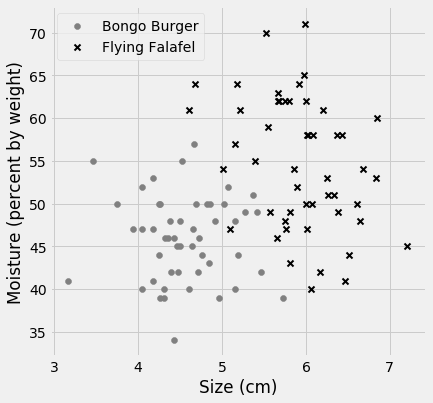
\includegraphics[scale=.6]{figures/falafel.png}
\end{center}

\begin{enumerate}
\subq{3} The two classes of falafel cannot be perfectly separated by a line on the plot above. Is it still appropriate to use k-nearest neighbors classification to classify the falafel?
    \vskip 0.1 in
    \solutionbubble \quad Yes, because k-nearest neighbors still works even if the data cannot be perfectly separated. \\[4pt]
    \bubble \quad Yes, because having individuals from different classes that overlap in their features allows you to use a higher value for k. \\[4pt]
    \bubble \quad Yes, because k-nearest neighbors transforms the data so that it can be separated by a decision boundary. \\[4pt]
    \bubble \quad No, because k-nearest neighbors does not work if the data cannot be perfectly separated. \\[4pt]
    \bubble \quad No, because the accuracy on the test set is guaranteed to be lower if the data cannot separated by a decision boundary. \\[4pt]

\clearpage
\textbf{Parts B and C refer to the information below.} \\
Natalia found another falafel on the ground. She wants to use the dataset we currently have to classify which restaurant the new falafel came from.  The following is an \textbf{unsorted } table of the seven pieces of falafel in our dataset closest (in terms of Euclidean distance between size and moisture content)  to the new piece of falafel:
\begin{center}
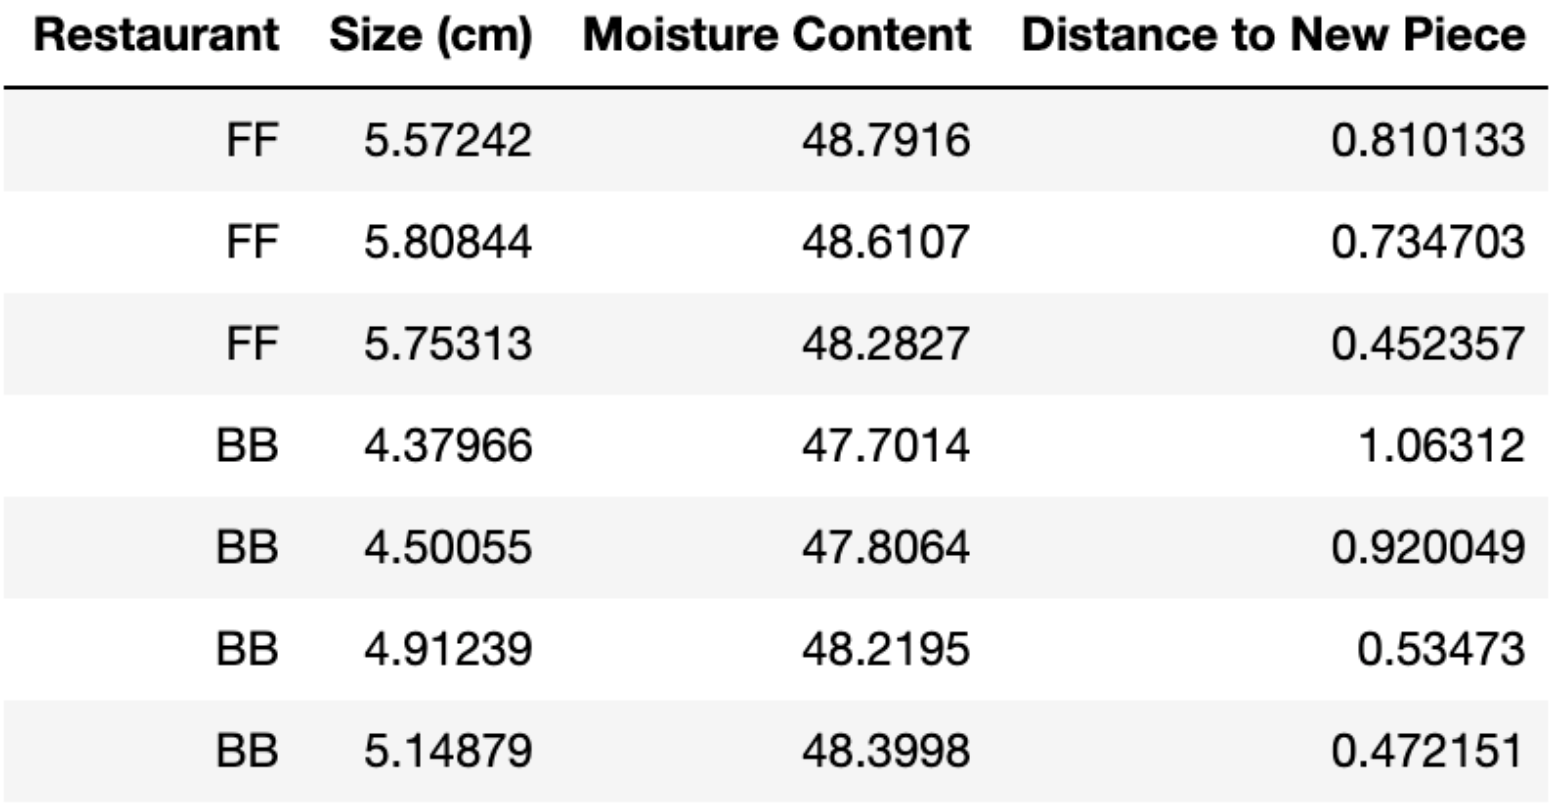
\includegraphics[scale=.34]{figures/falafel_nn.png}
\end{center}
\vskip0.1in
\subq{2} If we used a 3 nearest neighbor classifier, would we classify the new piece of falafel as coming from Bongo Burger or Flying Falafel?
\hspace{0.25in}\solutionbubble Bongo Burger\hspace{0.25in} \bubble Flying Falafel

\vskip .2in
\subq{2} If we used a 5 nearest neighbor classifier, would we classify the new piece of falafel as coming from Bongo Burger or Flying Falafel? 
\hspace{0.25in}\bubble Bongo Burger\hspace{0.25in} \solutionbubble Flying Falafel
\vskip0.1in
\subq{3} Shoumik is a visual learner and wrote out each step the classifier needs to perform on a different slip of paper and placed them on a desk. Before implementing the classifier Shoumik takes a break to teach his lab section. While he was gone, Shoumik's roommate rearranges the slips of paper while cleaning the desk, and now all the steps are out of order. Label the following steps as 1 ("do this first") to 6 ("do this last") in order to correctly implement a k nearest neighbors classifier. 
\vskip 0.1in
\solutionimage
{
{\underline{\qquad}} Take the top k rows of the sorted table\\[4pt]
{\underline{\qquad}} Calculate the classifier accuracy on all points in your test set\\[4pt]
{\underline{\qquad}} Classify the new point as the majority class in top k rows\\[4pt]
{\underline{\qquad}} Split the original data set into training and testing set\\[4pt]
{\underline{\qquad}} Sort the distances from smallest to largest\\[4pt]
{\underline{\qquad}} Calculate the distance between the new point and all points in the training set.
}
{
{\underline{\textbf{4}}} Take the top k rows of the sorted table\\[4pt]
{\underline{\textbf{6}}} Calculate the classifier accuracy on all points in your test set\\[4pt]
{\underline{\textbf{5}}} Classify the new point as the majority class in top k rows\\[4pt]
{\underline{\textbf{1}}} Split the original data set into training and testing set\\[4pt]
{\underline{\textbf{3}}} Sort the distances from smallest to largest\\[4pt]
{\underline{\textbf{2}}} Calculate the distance between the new point and all points in the training set.
}


\vskip 0.2in
\subq{2} Based on the scatter plot, which of the two features is more useful for differentiating falafel between the restaurants (e.g. if you could only use one feature to classify, which should you choose)? 
\vskip 0.03in
\hspace{0.25in}\bubble \quad moisture \hspace{0.25in} \solutionbubble \quad size
\vskip0.1in

\subq{3} The staff notice that falafel made in the morning are a different size than falafel made in the evening, as if restaurants are trying to conserve falafel batter at the end of the day. If you used a classifier trained on morning falafel to predict the label of an evening falafel, how might the accuracy of your classifier be affected? 
\begin{enumerate}
    \bubble \quad The test accuracy of your classifier would not change - you would do just as well using a classifier trained on morning falafel as a classifier trained on evening falafel.\\[2pt]
    \bubble \quad The test accuracy would increase because you are including more data.\\[2pt]
    \bubble \quad The test accuracy would increase because your accuracy would not depend on random variation in the morning falafel.\\[2pt]
    \solutionbubble \quad The test accuracy would decrease because the typical values of features for each restaurant might be different in the evening relative to the morning. 
\end{enumerate}

\vskip 0.2in
\subq{3} The staff decided to investigate evening falafel and created a new classifier using falafel collected in the evening. However, on the night of data collection Bongo Burger had a machine malfunction so the staff were only able to collect 10 BB falafel, and 90 FF falafel. A GSI tried many different values for \textit{k} (how many nearest neighbors to look at) when training their classifier, and noticed that above some value of \textit{k}, the classifier always classified any new falafel as coming from FF, regardless of its features. What is this value of \textit{k?} 
\vskip 0.1in
\begin{tabular}{l@{\hskip 0.5in}l@{\hskip 0.5in}l@{\hskip 0.5in}l}
\bubble \quad 11
&\bubble \quad 20 \\[10pt]
\solutionbubble \quad 21
&\bubble \quad 51
\end{tabular}



\end{enumerate}